\subsection{Overview}
\hspace{\parindent}Architectural design of the application is based on the three-layer model used in most applications. The three layers are the presentation layer, or frontend, the application layer, or middleware, and the data layer, or backend. Each of those layers does its own part of the job and communicates with other layers in order to present the correct information to the user.\\
The architecture is also a typical client-server implementation where server holds the data and the client is accessing it through requests (besides the offline mode where the user stored some of the data from the server locally and is accessing it without using online requests).\\
\newpage
\subsection{Frontend architecture}
\hspace{\parindent}Frontend part of the application is using viewmodels, which are more commonly known as \textbf{model-view-viewmodel} architecture.\\ \\
The base of the Android app technology is the Android Compose, which uses different approach to the app development, as it draws specific components based on the state that the app is in. This makes for much more lightweight app, as the activity or intent of the Android app is much less frequently changed as only some of the components that are being drawn out on the screen are being interchanged, which saves a lot of time and resources. This approach also allows for code reusability as components can be used in either completely identical shapes, or just slightly altered depending on the use.\\ \\
This is where the viewmodel architecture comes in. Instead of directly handling the data and communicating with the data layer of the application, which in this case is done through the middleware, the frontend has additional sub layer which handles all the data, communication, and calculations of which parts of the interface should be shown. There are many advantages to this, with the main ones being complete independent handling of the communication and the presentation.\\ \\
Making big changes or adding additional functions in the middle of the app development can exponentially increase the production time and can quite often lead to rewriting the same parts of the code multiple times. Viewmodel architecture provides a certain kind of stability of the code, as adding additional function will usually mean writing either only the presentational part or the communication part, and then just connecting it with other already existing functions. It dramatically improves clarity and speed of development once everything is set up. Lastly, detecting bugs and unintended behaviour in the app is far easier, as we always know in which layer the problem is located. This makes it not only easier to find, but also easier to fix, as there is a good chance that we are only going to have to change a small part of the code, assuming that the other part is written correctly. In other types of architectures this often leads to rewriting entire parts of the frontend.\\ \\
One of the main disadvantages of this model is it's complexity, as there is another additional layer of communication in which the data needs to be handled and adapted in order to be passed through. This of course increases the time of development and the possibility of bugs, but if everything is done correctly, it provides a great tradeoff.\\

Almost every screen/activity has it's own view model, with the focus being on ones that have the most communication with the backend. The list of all the activities and their respective viewmodels is the following:
\begin{itemize}
\item Main Activity		
\item Trip Activity	 - Trip View Model
\item Trips Screen	 - Trips View Model
\item Trip Creation Activity	- Trip Creation View Model
\item Map Screen	 - Map View Model
\item Location Screen	 - Location View Model
\item Location Selection Screen	- Location Selection View Model
\item Home Screen	 - Home View Model
\item Google Place Screen	 - Google Place View Model
\item Login Activity
\item Inspiration Activity
\item Explore Screen
\item Around Me Activity
\item Active Trip Activity
\item Profile Screen
\end{itemize}
Other types of design elements included in front development, besides the common ones used in pretty much every single app, include the following:
\begin{itemize}
\item Bars
\item Buttons
\item Cards
\item Switches
\item Icons
\item Images
\item Map
\end{itemize}
The general design and look of the UI is shown in more detail in the Chapter 4 of the document.
\newpage

\subsection{Backend architecture}
\subsubsection{User database}

\hspace{\parindent}As previously mentioned, user database is located in the Google Firestore service. This service uses real-time NoSQL database. This database is organized in collection->document system. Everything starts with one collection, which can hold as many documents (entities) as possible. Each document can have an unlimited number of attribute fields, which can be with a specified type or without one, and at most one collection. Then the cycle repeats again.\\ \\
Working with NoSQL has its advantages when it doesn't have a lot of relational and connected data. We can extract only the small amount of data we want, it is very fast, and also very efficient. Since accounts are not connected in any way, using NoSQL database  seemed like a viable choice since it saves our users time and data. \\ \\
The architecture of this database is the following: the first collection contains all the users as their unique IDs, where they are represented by a document. The first level of the document holds only the info of the display name and the ID.  The second collection is made for storing user preferences, and every user has their own. In that collection there is a document that holds all of the parameters needed for the user's usage of the app, such as colour mode, economy level, thumbnail URL; and two optional ones, real name and real surname
\\ \\
The following figure represents the structure of the explained database.\\
\begin{figure}[!htb]
\centering
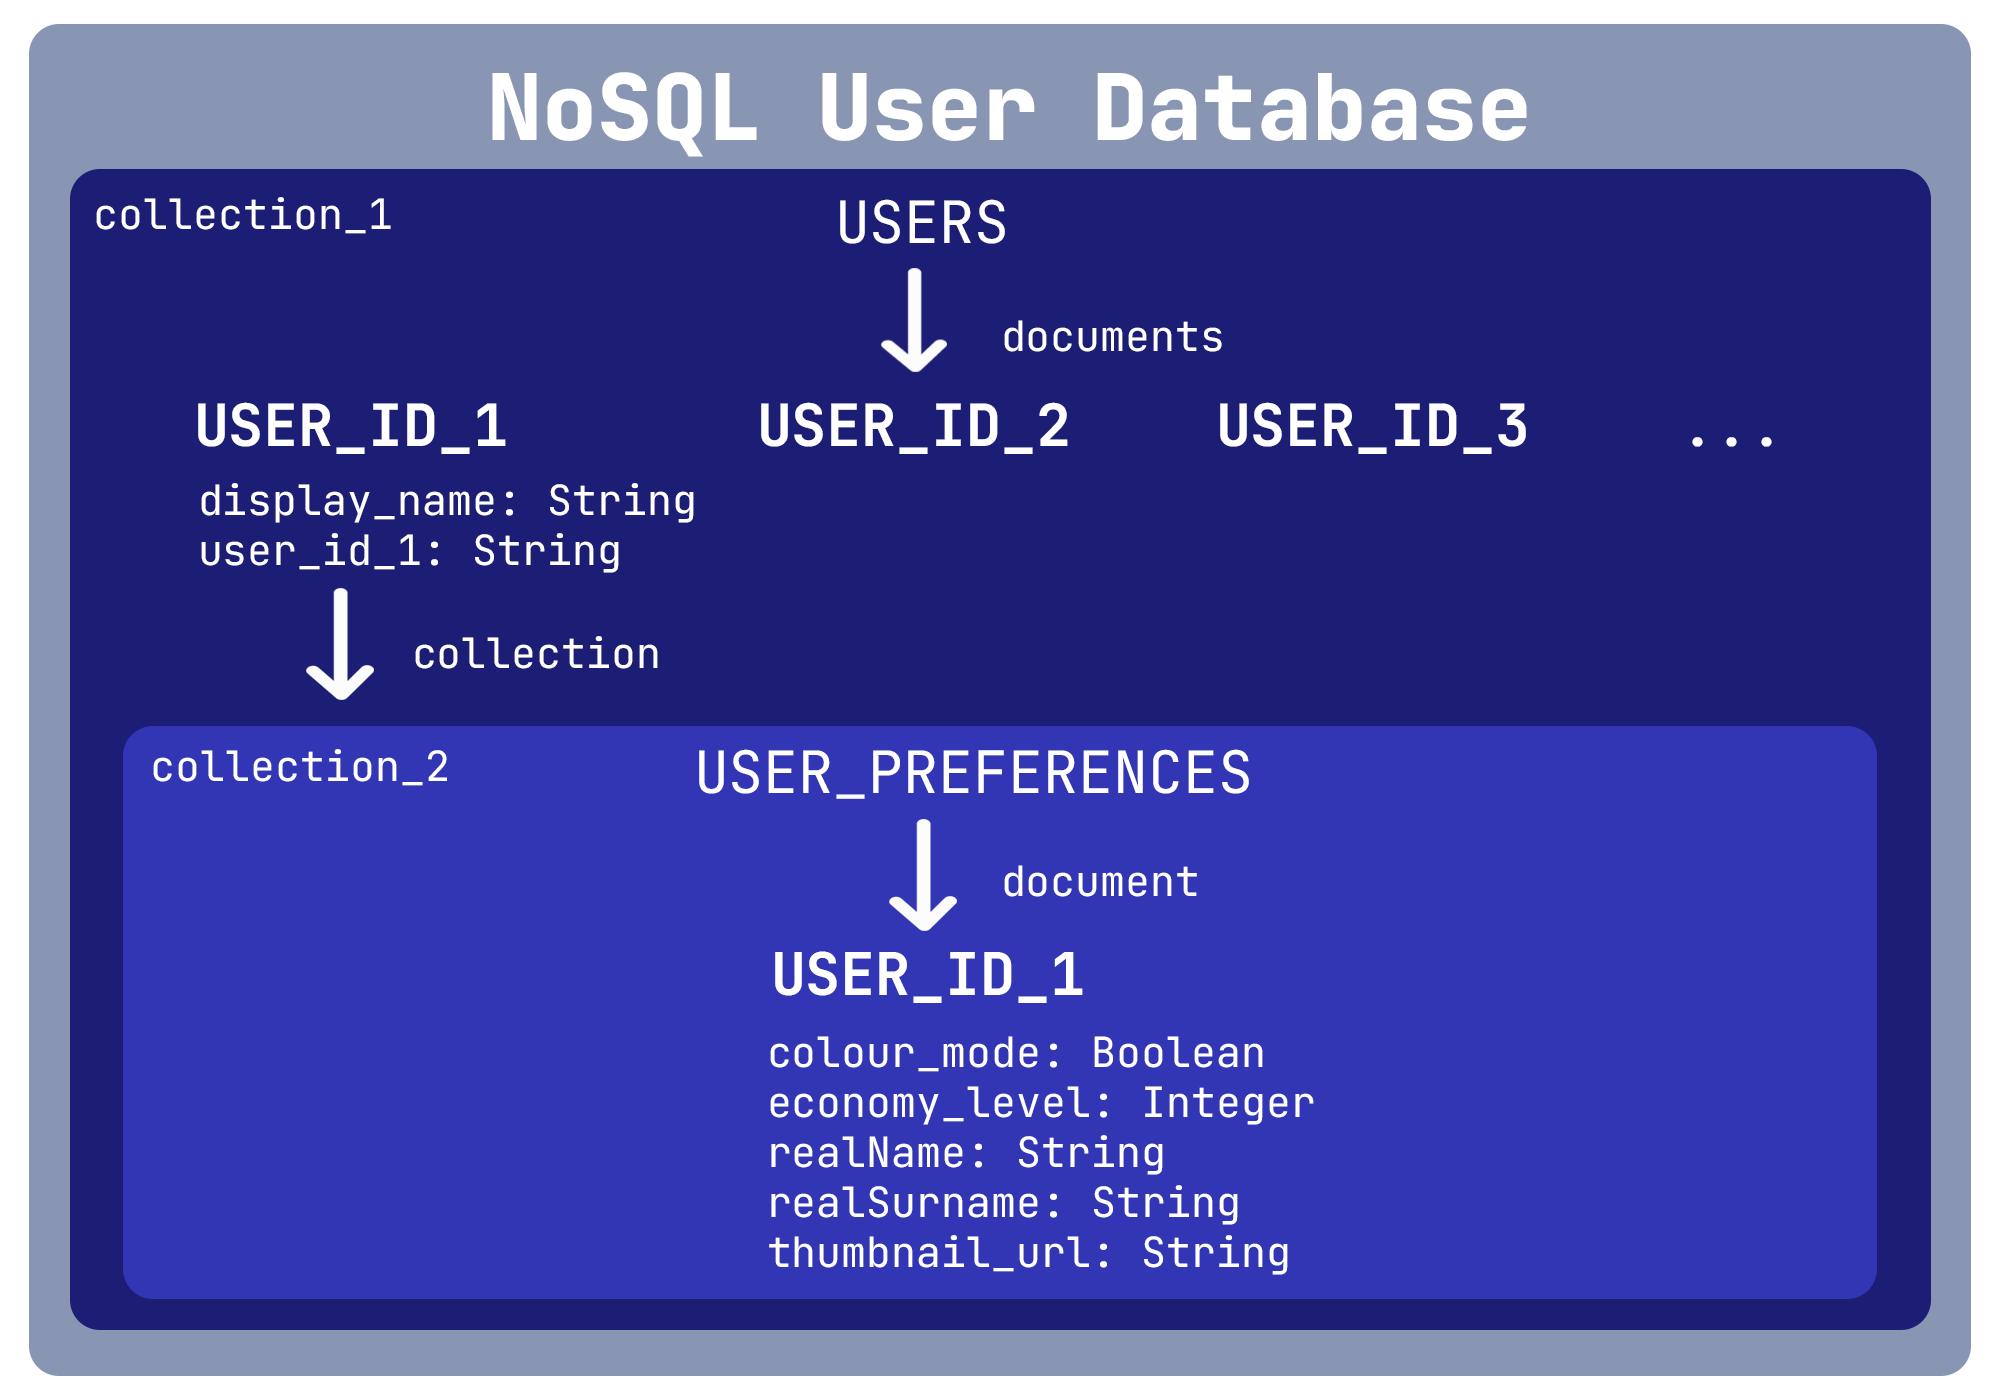
\includegraphics[width=\textwidth]{../Images/NoSQLStructurePNG.png}
\caption{\label{fig:dbapiuser}\textbf{Structure of the NoSQL user database}}
\end{figure}
\newpage

\subsubsection{Trips database}
\hspace{\parindent}Database regarding trips has several different parts that make the whole system work. The most integral part of every trip are destinations. There are two types of destinations in the database - destinations retrieved from Google Places API and user created destinations.\\ \\
When adding a destination to the trip, users can either find a destination using Google Places API, or if they are not satisfied with the search, they can create their own destination, with a unique name and a location on the map. This destination can then be provided with a specific name, GPS coordinates, rating, and an thumbnail image. Newly added destinations receive an ID generated by the backend, while Google Places destinations have their own unique ID, which has a different form and shape. Users are always going to be urged to use already existent destinations, so unless there is not a really specific location in question, they would have no need to create their own, especially since the Google database is quite large.\\ \\

\begin{figure}[!htb]
\centering
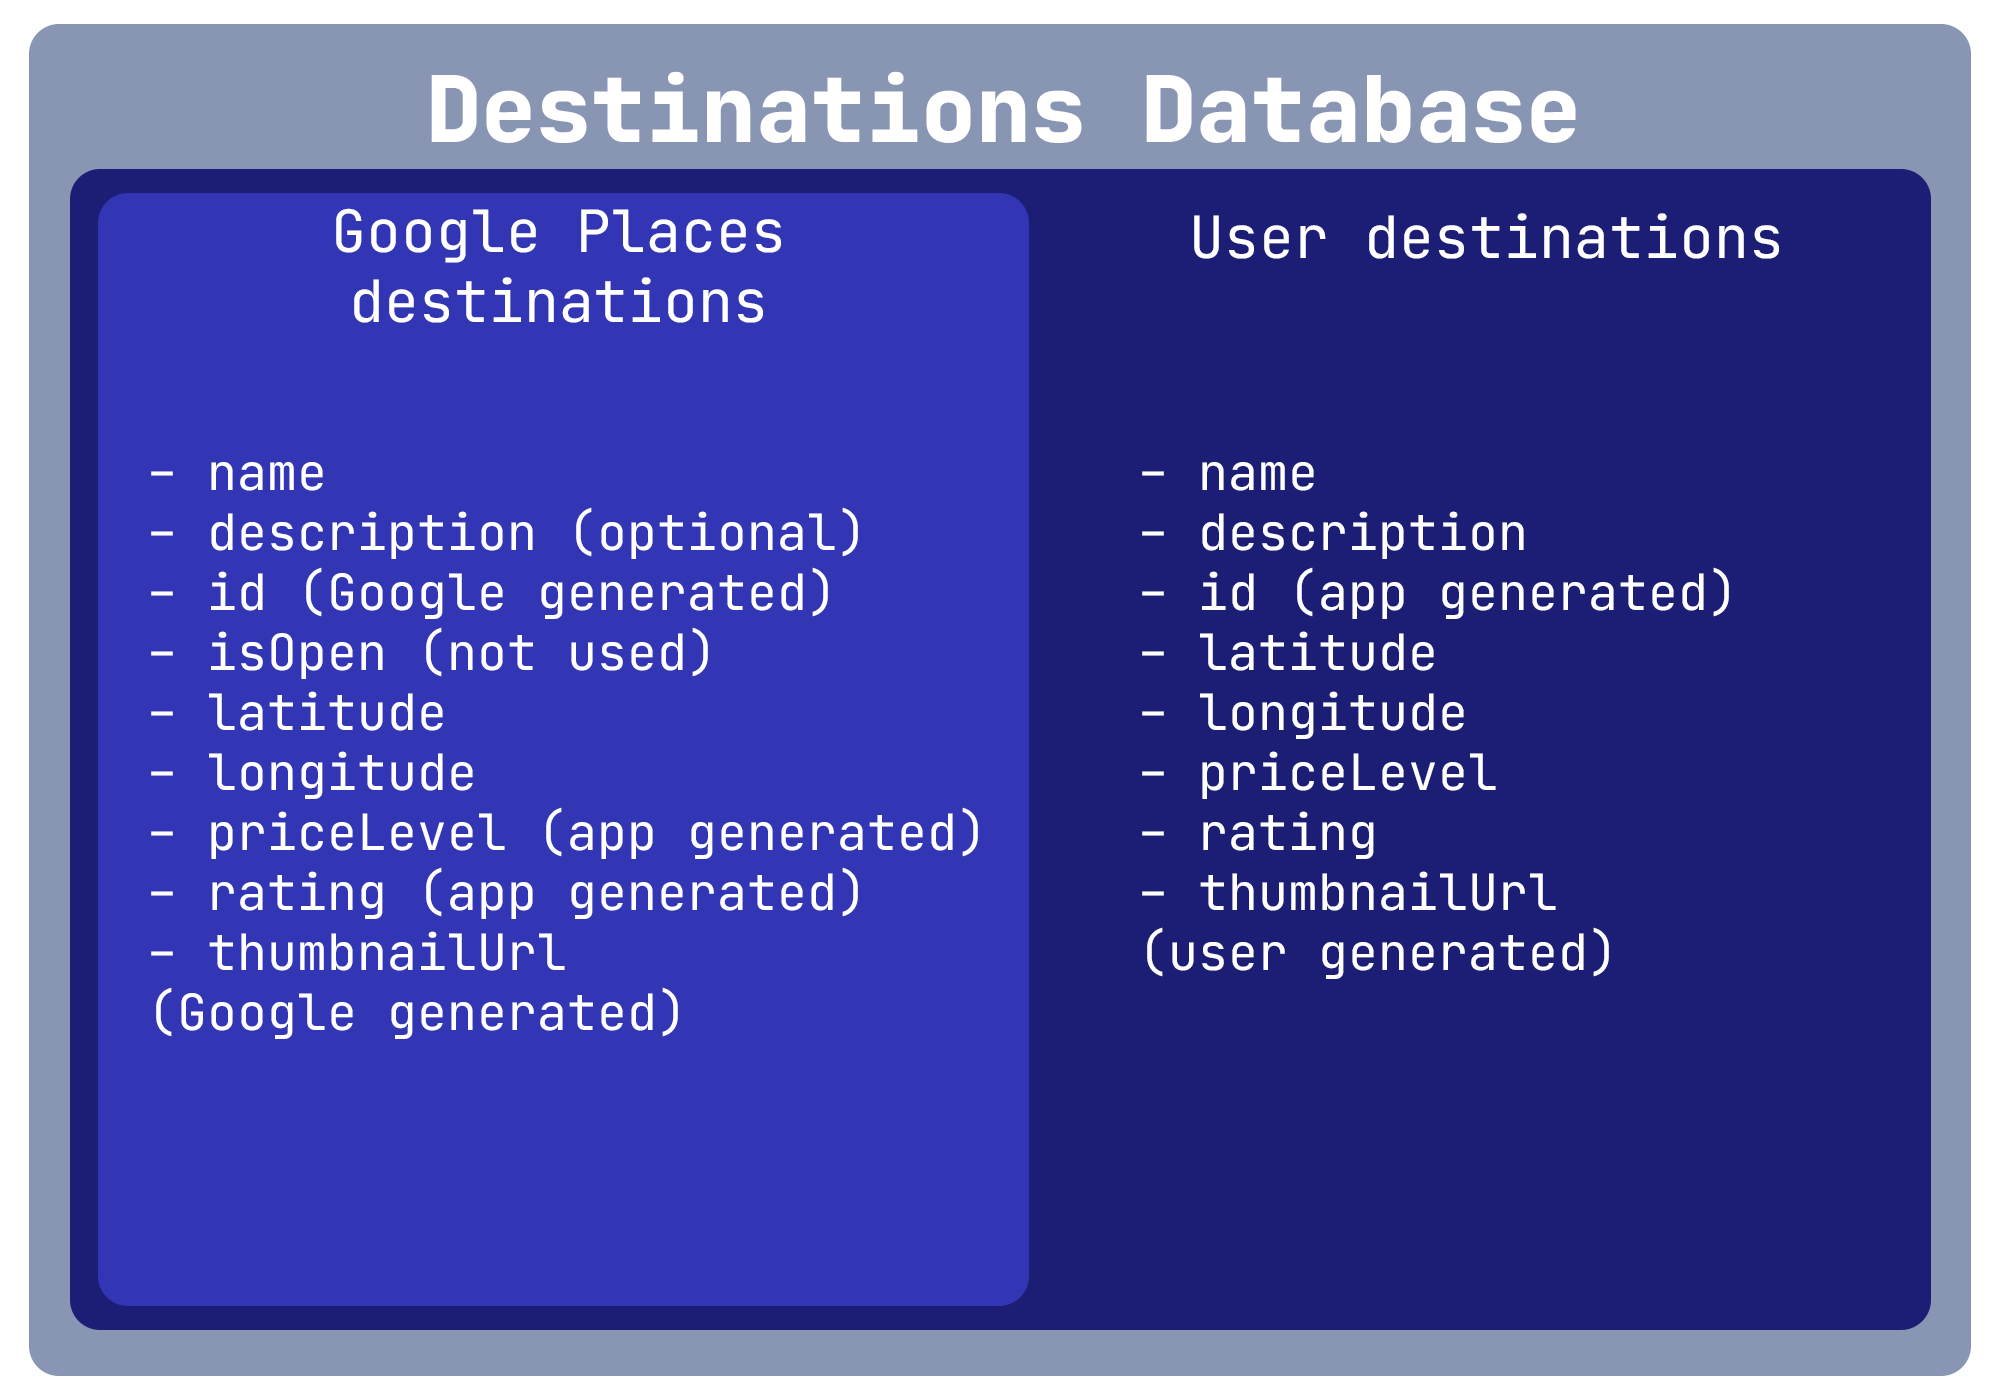
\includegraphics[width=\textwidth]{../Images/DestinationsStructurePNG.png}
\caption{\label{fig:dbapiuser}\textbf{Structure of the "Destination" entities}}
\end{figure}
\newpage

Trips structure are much more complex and detailed. Every trip is defined by several important attributes. Besides the basic information like name, id, description, and thumbnail URL, trips are mainly defined by destinations. Central point destination is the most important point of the trip, which necessarily doesn't have to be a beginning or an ending destination. Then for every single day of the trip there could be one or more destinations defined. Along with the regular destination attributes, those destinations feature the distance to the next destination (both in minutes and kilometers) taken with the recommended mean of transport, which is calculated through Google Maps and Places APIs. Those destinations also feature approximate hours of arrival and a recommended time to be spent there so that a plan could be fully followed. Every destination can also feature notes which could give users additional information about it or just provide some tips on what to do and what to see. A list of image URLs can also be added for every specific destination in the list. \\ \\
Besides all of the destinations and the basic info, trip entity also features creator of the trip, creation date, recommended season of travel, rating, and public boolean, which defines whether the trip is private (and therefore hidden from other users) or public (and can be seen by everyone). \\
\begin{figure}[!htb]
\centering
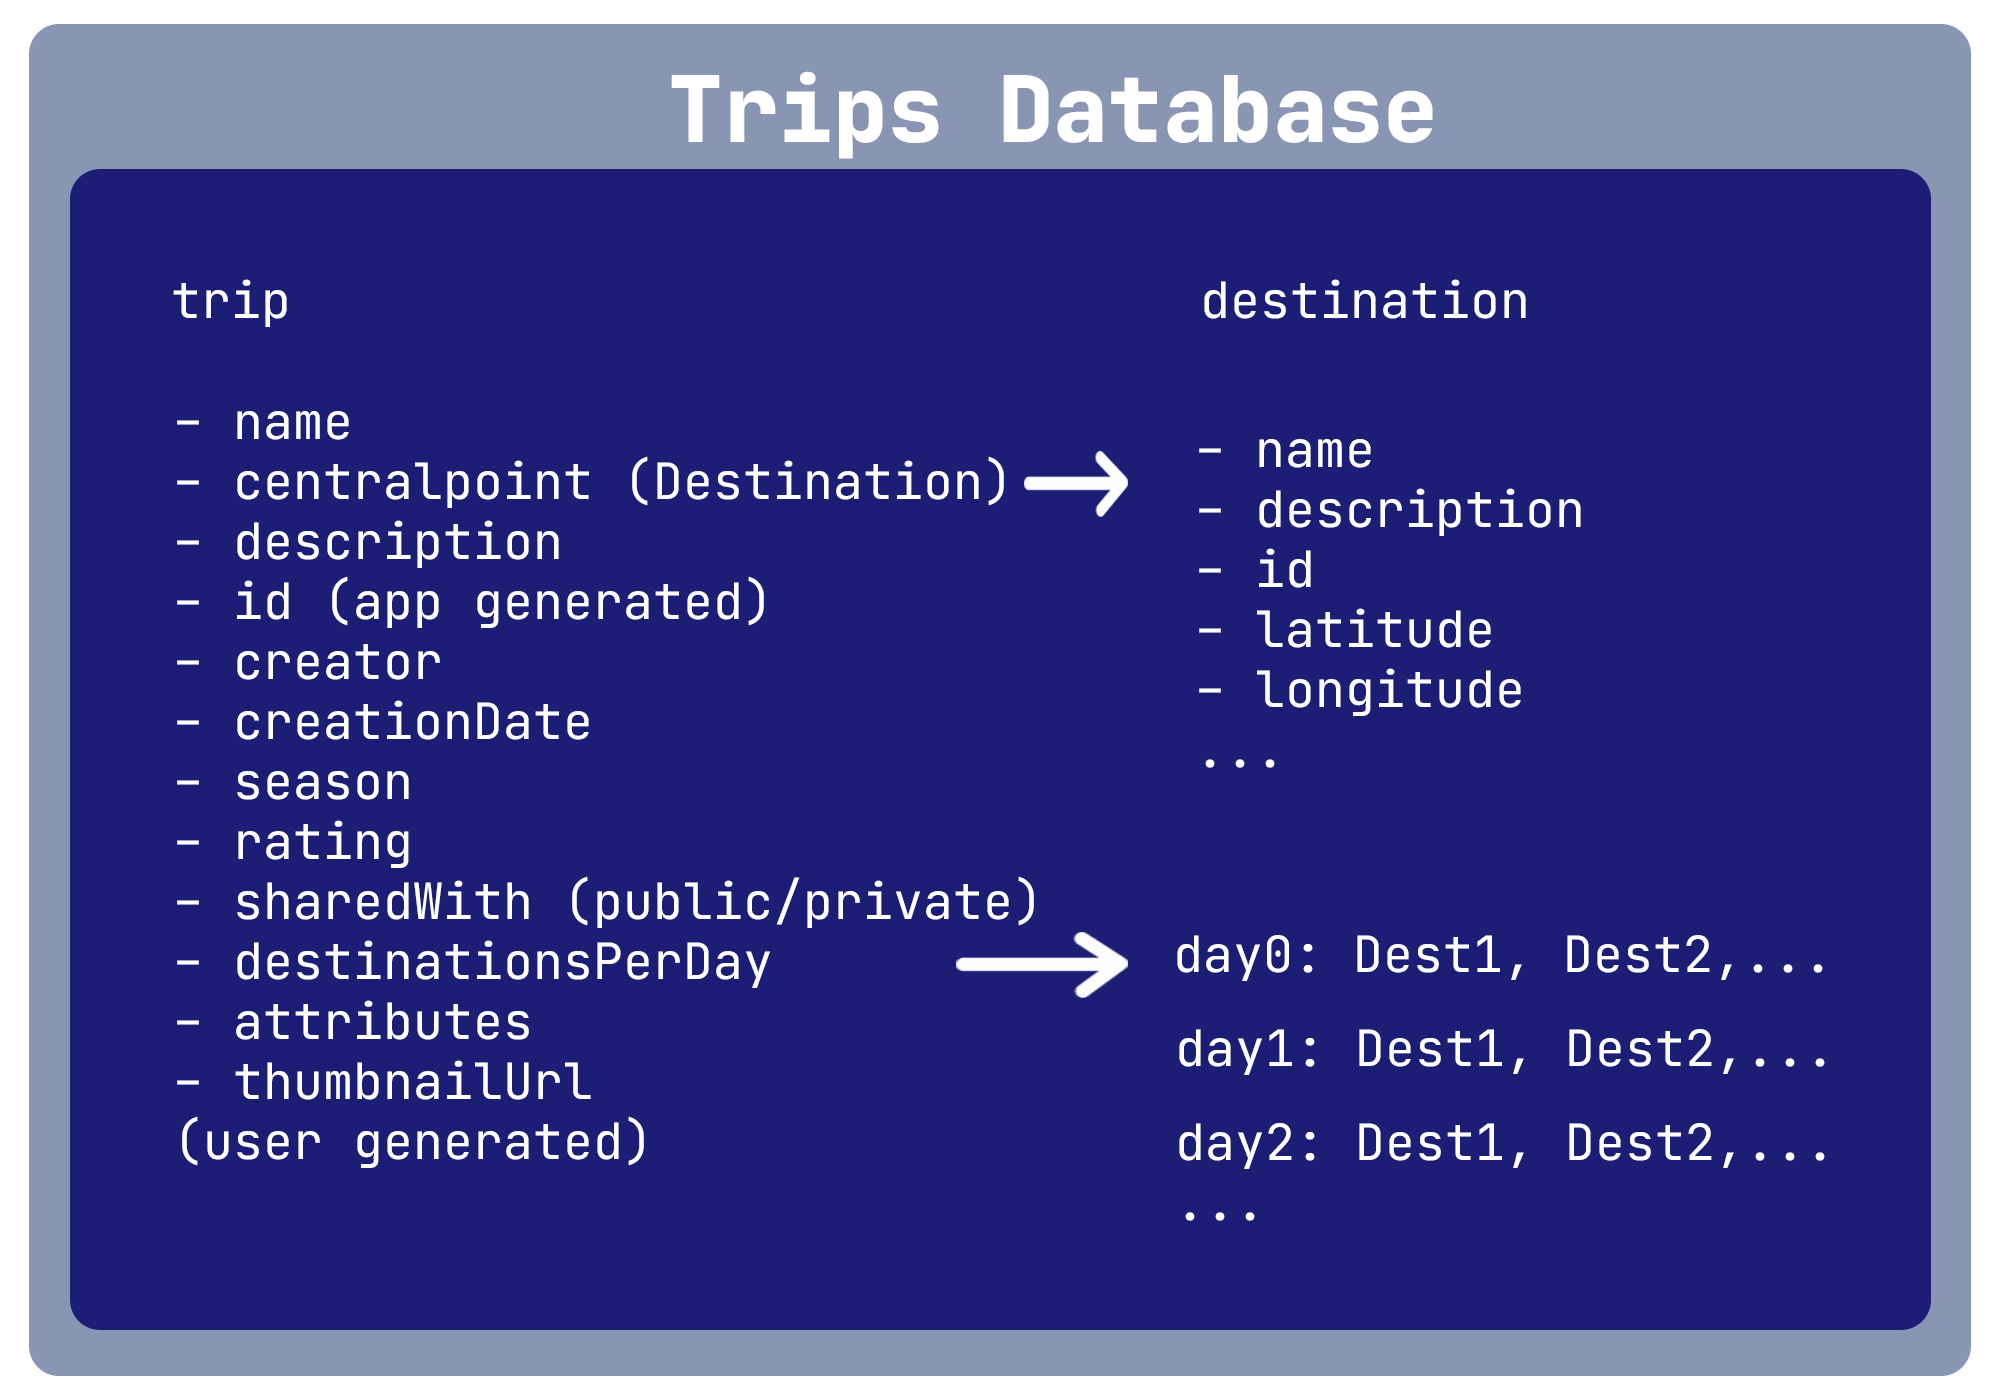
\includegraphics[width=\textwidth]{../Images/TripsStructurePNG.png}
\caption{\label{fig:dbapiuser}\textbf{Structure of the "Trip" entities}}
\end{figure}
\newpage


\subsection{Middleware architecture}
\hspace{\parindent}In order to connect the data on the server to the screen of the phone and to allow the user to properly see the data, we have implemented a complicated layer of functions and classes in order to create easy-to-use and esthetically pleasing experience for the user. In this section the most important functions of this layer, and everything that does not belong to the frontend and backend will be explained.\\ \\
In general, it works as a separator or a controller of the three-layer infrastructure that is being used by the app.
\subsubsection{Communication with the backend}
\hspace{\parindent}App comunicates with the backend through the queries. After user's input, they are generated within the app, and the query is sent to the database. Database then collects all the needed data and sends it back to the application in the form of JSON files, which are easily readable and are rather simple to manipulate. 

\subsubsection{Handling unexpected actions}
\hspace{\parindent}There are several instances in which the unexpected behaviour of the app or the phone can cause users to lose a lot of their previous work. As creating a new trip from scratch can be a long process, especially for longer trips, there is always a problem of consistency. If the user visits some other apps in the meantime, the risk of 'Polaris' app changing lifecycle state can destroy all of the previous work. The same can also happen with the phone's battery being depleted or if the user accidentally closes the app.\\ \\

The solution of this problem is found in the premature saving of the trip. Every time the user leaves the trip unfinished or exits the app without either saving or discarding the trip, the app will save the trip with the "unfinished" attribute. This means that the trip will exist just like normal trips, but will not be published in neither private or public mode. The reason for that is that the trip might not even have the most basic attributes like name, which is a crucial attribute for the trip to be published, but is quite often left as the final piece of the puzzle when being created by the user.\\ \\

This way whenever the users return to the library of created/saved trips, they will found the previously unfinished trip and will be able to continue from where they left off. The middleware handles this part on its own, storing the trip in the database and taking care of all of the necessary actions, so the user doesn't have to worry about storing or fetching the trip. 

\subsection{Runtime view}

\hspace{\parindent}In the following section, sequence diagrams that represent the most important use cases are shown and explained in detail. We have focused only on the most commonly used use cases in the app, as well as their crucial parts. We do not go into too much detail when it comes to specific parts of interaction between the layers, but rather want to present the vague idea and how it all works.
\newpage
\subsubsection{Create a trip}

\hspace{\parindent}Create a trip use case starts with opening the app and pressing on the "Create a trip" button. A new screen opens up which allows us to change certain attributes about the trip and add different destinations. Every trip needs to have a name, which doesn't have to be unique, since there is an ID that is automatically allocated to the every trip. Every trip needs to have at least two destinations. We can search through destinations via the search bar or by using the interactive map and selecting a destination from the map. After selecting a destination, we add it to the trip. Destinations can be reordered and removed from the trip at any time, which is not shown in the diagram due to simplicity and concision. The price level of the trip should also be defined before saving the trip. Trip can also be discarded. In the end, if the user is satisfied with its trip, they can publish it in which case it will be stored directly in the database. Local database is not used for storing unpublished trips, since this would mean that by losing local data, all of the unpublished trips would be lost. All of the trips are stored in the online database and are can be found by other users only if published.  
\begin{figure}[!htb]
\centering
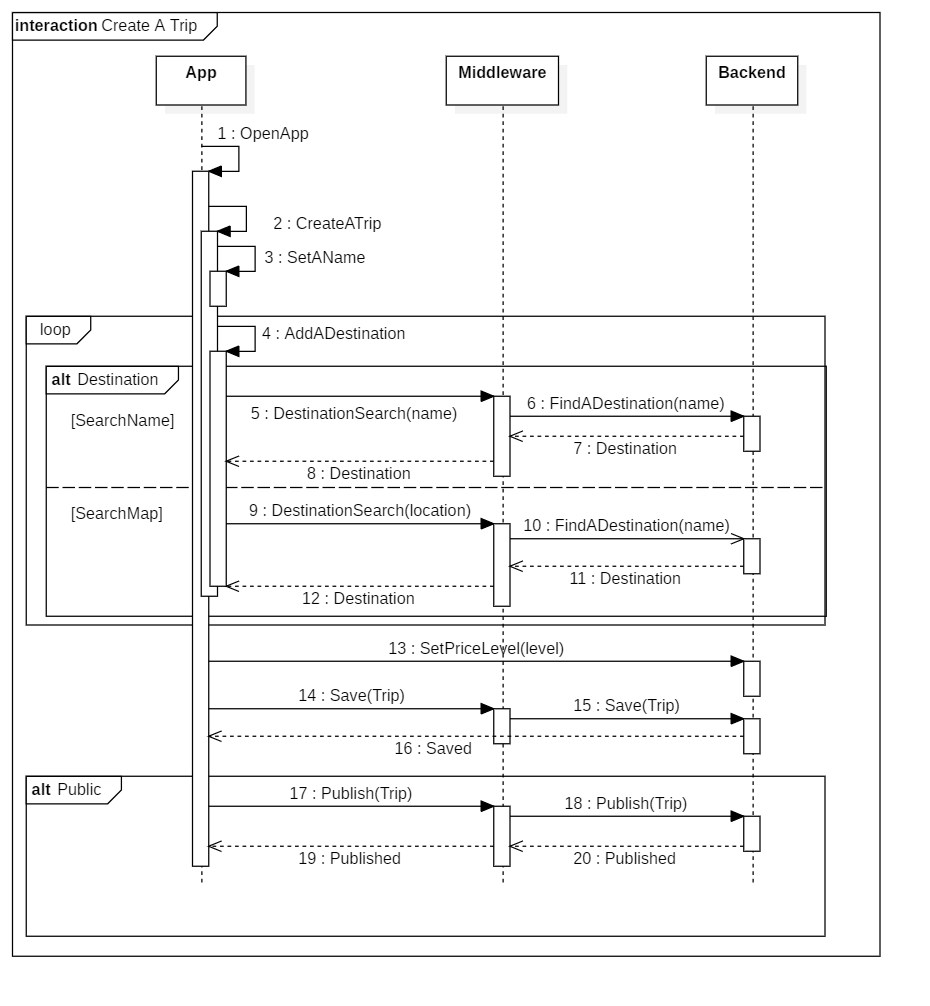
\includegraphics[width=0.9\textwidth]{../Graphs/Sequence1_Create_A_Trip.png}
\caption{\label{fig:dbapiuser}\textbf{Sequence diagram 1 - Create a Trip}}
\end{figure}
\newpage
\subsubsection{Edit a trip}

\hspace{\parindent}Edit a trip use case starts with opening the app and choosing one of two ways of searching for a trip. One way is searching for a trip name/ID directly through the search bar, and another is by searching for a trip on the interactive map. After the trip is found, it is somewhat "copied" to the instance of the user. User can then edit every single bit of the trip - change the name, change the price level, and add/remove destinations (again, destination removal is not shown in the graph due to simplicity). Finally the user can choose to save the trip without publishing it, or publish it so that everyone else is able to find it. Either way, the trip gets a brand new ID only if it has been changed in any way (changing only the trip name and/or price level is not regarded as a change). Again, due to data safety, in either case it is stored online.\\
\begin{figure}[!htb]
\centering
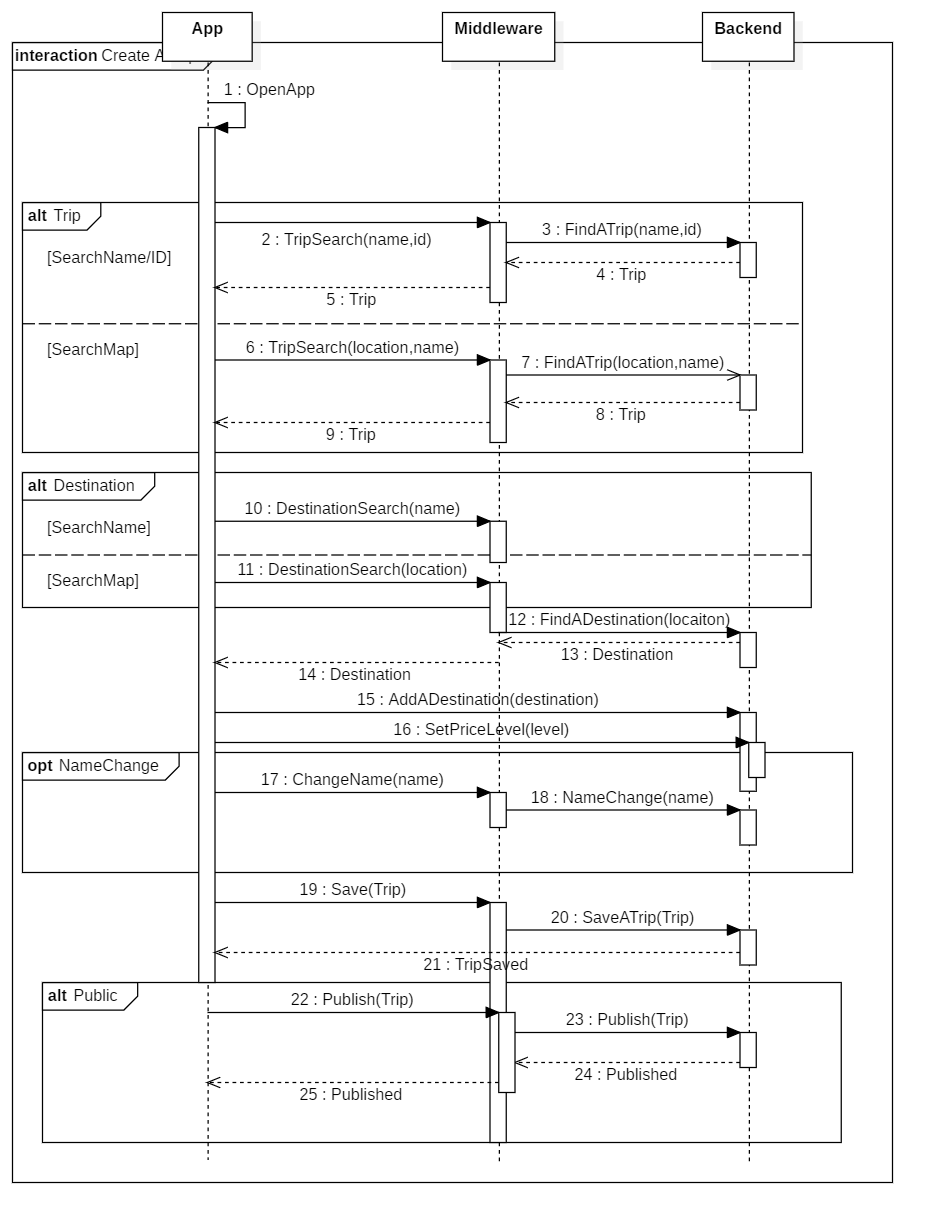
\includegraphics[width=0.8\textwidth]{../Graphs/Sequence2_Edit_A_Trip.png}
\caption{\label{fig:dbapiuser}\textbf{Sequence diagram 2 - Edit a Trip}}
\end{figure}
\newpage
\subsubsection{Add a destination}

\hspace{\parindent}Add a destination use case starts with opening the app and choosing one of two ways of adding destination - either by using the dynamic Google Maps API, or by using a search function which searches for specific places and locations in the Google database. By using a Google Maps way, the user can specify the exact location, while by using the search way, the user can pick of the previous existing locations in the database. After picking a location, the user can change a name and/or add an specific image of this location. This way the user is allowed to personalize locations for their trip needs. After saving all of the data in the form of a destination, the new destination is published and can be found by other users and added to their trips. There are no local and unpublished destinations.\\
\begin{figure}[!htb]
\centering
\includegraphics[width=0.9\textwidth]{../Graphs/Sequence3_Add_A_Destination.png}
\caption{\label{fig:dbapiuser}\textbf{Sequence diagram 3 - Add a destination}}
\end{figure}
\newpage
\subsubsection{Search for a trip/explore}
\newpage
\subsection{Design constraints}
\subsubsection{Hardware limitations}
\hspace{\parindent}As previously mentioned, the application is currently only made for Android OS, using native Android development. iOS devices, as well as Windows Mobile OS devices, and Web/Desktop version of the software is currently not available.\\ \\
The application will only work on Android devices that support Android 7.0(Nougat) which is Android API 24 or above, due to security reasons, and due to specific software features that are not available in the previous versions of this software. As this version is over six years old, and vast majority (over 90\%) of Android users are currently running this or higher version, we estimated this to be a viable choice for the lowest supported version. As of right now, the latest version of the Android OS is 12 or API level 31, which is also the target build for the app.\\ \\
Device is use is required to have access to the Internet for the initial(and any subsequent) login, and for the initial data fetching. The Internet connection is not required when using the application in offline mode, after the desired trips have been downloaded and locally stored. In case of using the application without Internet connection, the full features of the app may not be available to the user.

\subsubsection{Privacy limitations}
\hspace{\parindent}The user is not required to insert any personal information in the app, besides their email or social media account which is necessary for login. This email will not be visible to the other users. The user may provide his real name and surname, which would make them easier to find by other users, although the primary identification will still be in the form of username, which is initially set by the user. User may also provide an image that will be used for the thumbnail of their account, which is also optional. User's comments on trips will be seen by everyone if the trip has been made public. If the user wants to keep the comments to themselves, it is possible to leave the trip unpublished.
